% !TEX program = pdflatex
%% =====================================================================
%%  Defensa de TFM — Comparación de codificadores visuales en Diffusion Policy
%%  Compilar:  latexmk -pdf beamer.tex
%%  Todas las cifras proceden de la memoria (memoria/main.tex y secciones/).
%% =====================================================================
\documentclass[aspectratio=169,11pt]{beamer}

\usepackage[T1]{fontenc}
\usepackage[utf8]{inputenc}
\IfFileExists{spanish.ldf}
  {\usepackage[spanish,es-nodecimaldot,es-noshorthands]{babel}}
  {\usepackage[english]{babel}\PackageWarning{beamer}{babel-spanish no instalado}}

\usepackage[oxford,serif]{talkstyle}
\usepackage{amsmath,amssymb,bm}
\usepackage{booktabs}
\usepackage{siunitx}
\usepackage{graphicx}
\usepackage{appendixnumberbeamer}
%% notacion.tex — macros de la charla, alineadas con la memoria (cap. Metodologia)

\DeclareMathOperator*{\argmin}{arg\,min}
\DeclareMathOperator*{\argmax}{arg\,max}

\newcommand{\E}{\mathbb{E}}
\newcommand{\R}{\mathbb{R}}
\newcommand{\norm}[1]{\left\lVert #1 \right\rVert}
\newcommand{\abs}[1]{\left\lvert #1 \right\rvert}
\newcommand{\est}[1]{\hat{#1}}

% Notacion de Diffusion Policy, identica a la de la memoria
\newcommand{\Obs}{\mathbf{O}_t}            % observaciones de los ultimos T_o instantes
\newcommand{\Act}[1]{\mathbf{A}^{#1}_t}    % secuencia de T_p acciones futuras
\newcommand{\rnet}{\epsilon_\theta}        % red que predice el ruido
\newcommand{\rui}{\epsilon^k}              % ruido inyectado en el paso de difusion k

% "donde ..." debajo de una ecuacion, en gris y pequeno
\newcommand{\donde}[1]{\par\vspace{0.35em}{\small\color{tsMute}donde #1}}


\graphicspath{{../img/}{img/}}
\sisetup{detect-all, output-decimal-marker={,}, group-digits=false}

\title{Codificadores visuales en Diffusion Policy}
\subtitle{Protocolo con prueba disjunta, rendimiento y coste: cinco bloques visuales en Push-T}
\author{Moises Britez}
\institute{Máster en Análisis de Datos en Ingeniería · Tecnun · Director: Diego Borro}
\date{Donostia-San Sebastián · septiembre de 2026}
\makeatletter
\def\insertshortauthor{M. Britez}
\def\insertshorttitle{Codificadores visuales en Diffusion Policy}
\makeatother

\begin{document}

% ---------------------------------------------------------------- portada
\begin{frame}[plain,noframenumbering]
  \titlepage
\end{frame}

\section{El problema}

% ---------------------------------------------------------------- 1. gancho
\begin{frame}{El codificador visual decide qué llega al generador}
  \begin{columns}[T,onlytextwidth]
    \begin{column}{0.56\textwidth}
      \begin{itemize}
        \item Imitación: la acción se aprende de demostraciones humanas.
        \item Misma imagen, rutas distintas: la regresión las promedia y descarrila.
      \end{itemize}
      \src{Florence \emph{et al.} (2021); Chi \emph{et al.} (2025).}
    \end{column}
    \begin{column}{0.40\textwidth}
      \begin{keypoint}
        Y todo pasa antes por un cuello de botella: el \hl{codificador visual}.
      \end{keypoint}
    \end{column}
  \end{columns}
\end{frame}

% ---------------------------------------------------------------- 2. hueco
\begin{frame}{Diffusion Policy resolvió el generador; el codificador sigue sin decidirse}
  \begin{itemize}
    \item Difusión condicionada: acciones multimodales sin promediar.
    \item Después se cambió el generador y la entrada.
    \item En Push-T, nadie contrasta ResNet-18, DINOv2 y CLIP bajo el mismo protocolo.
  \end{itemize}
  \begin{keypoint}
    \textbf{Pregunta:} con \num{90} demostraciones, ¿preentrenar?
    ¿\hl{Congelar} o \hl{ajustar}?
  \end{keypoint}
\end{frame}

% ---------------------------------------------------------------- 3. la charla en una diapositiva
\begin{frame}{La respuesta corta: el preentrenamiento de ImageNet estorba aquí}
  \begin{enumerate}
    \item \textbf{Diseño.} Cinco bloques visuales en la misma política; lo demás, idéntico.
    \item \textbf{Resultado} sobre \num{200} condiciones nunca consultadas: desde cero
          \hl{\num{0.872}}; ResNet congelada \num{0.649}; ResNet ajustada \num{0.586};
          DINOv2 \num{0.578}; CLIP \num{0.490}.
    \item \textbf{Coste.} La línea base, además, entre \num{1.4} y \num{9.2} veces más
          barata por época.
  \end{enumerate}
  \takeaway{Peor y más caro: no hay compromiso que negociar.}
\end{frame}

\section{Diseño experimental}

% ---------------------------------------------------------------- 4. la tarea
\begin{frame}{Push-T: contacto intermitente y varias soluciones válidas}
  \begin{columns}[T,onlytextwidth]
    \begin{column}{0.52\textwidth}
      \begin{itemize}
        \item Empujar una pieza en T hasta la silueta objetivo.
        \item Imagen cenital \num{96}$\times$\num{96} y posición del efector.
        \item \num{206} demostraciones, \num{25650} transiciones, \num{90} episodios de
              entrenamiento.
      \end{itemize}
      \src{Chi \emph{et al.} (2025).}
    \end{column}
    \begin{column}{0.44\textwidth}
      \begin{keypoint}
        \hl{Pocas demostraciones}: el régimen donde el preentrenamiento debería ayudar.
      \end{keypoint}
    \end{column}
  \end{columns}
\end{frame}

% ---------------------------------------------------------------- 5. ecuacion
\begin{frame}{La política aprende a predecir el ruido, condicionada por la imagen}
  \[
    \mathcal{L} \;=\;
    \E\Big[\,\big\lVert\,
      \ann{\rui}{ruido inyectado}
      \;-\;
      \rnet\big(\hl{\Obs},\; \Act{0}+\rui,\; k\big)
    \,\big\rVert^2\Big]
  \]
  \donde{$\Obs$ son las $T_o=2$ observaciones y $\Act{0}$ la secuencia de $T_p=16$
    acciones reales.}
  \pause
  \begin{keypoint}
    $\Obs$ entra como \hl{condicionamiento}, no se genera. Lo que el codificador no
    ponga en ese vector de \num{512} componentes, el generador no lo tiene.
  \end{keypoint}
\end{frame}

% ---------------------------------------------------------------- 6. variantes
\begin{frame}{Cinco codificadores, un solo factor manipulado}
  \begin{center}
  \begin{tabular}{llll S[table-format=3.0]}
    \toprule
    & Codificador & Pesos iniciales & Estrategia & {Entrenables (M)} \\
    \midrule
    \textbf{V0} & ResNet-18       & aleatorios  & desde cero  & 288 \\
    V1 & ResNet-18       & ImageNet-1k & congelado   & 277 \\
    V2 & ResNet-18       & ImageNet-1k & ajuste fino & 288 \\
    \fade{V3} & \fade{DINOv2 ViT-S/14} & \fade{LVD-142M} & \fade{congelado} & \fade{277} \\
    \fade{V4} & \fade{CLIP ViT-B/16}   & \fade{WIT-400M} & \fade{congelado} & \fade{277} \\
    \bottomrule
  \end{tabular}
  \end{center}
  \src{V3 y V4 siguen en ejecución: esta charla cubre las tres variantes convolucionales.}
  \takeaway{Constantes: generador, hiperparámetros, semilla \num{42}, partición y
    protocolo de evaluación.}
\end{frame}

% ---------------------------------------------------------------- 7. evaluacion
\begin{frame}{Cómo se mide}
  \begin{itemize}
    \item Cada \num{50} épocas, \num{50} episodios de bucle cerrado, semillas reservadas.
    \item Puntuación: cobertura máxima del objetivo, saturada en $\tau=\num{0.95}$.
    \item Se guarda el punto de control de mayor puntuación media.
  \end{itemize}
  \begin{keypoint}
    Esos episodios \hl{seleccionan} el modelo: no son prueba independiente.
  \end{keypoint}
  \vspace{2mm}
  Por eso, con los cinco puntos de control ya congelados, se midió \emph{una sola vez}
  sobre \num{200} condiciones del bloque \numrange{200000}{200199}, bajo un protocolo
  escrito y registrado antes de ejecutarlo.
\end{frame}

\section{Resultados}

% ---------------------------------------------------------------- 8. figura score
\begin{frame}{La línea base se estabiliza cerca de \num{0.86}; las preentrenadas retroceden}
  \centering
  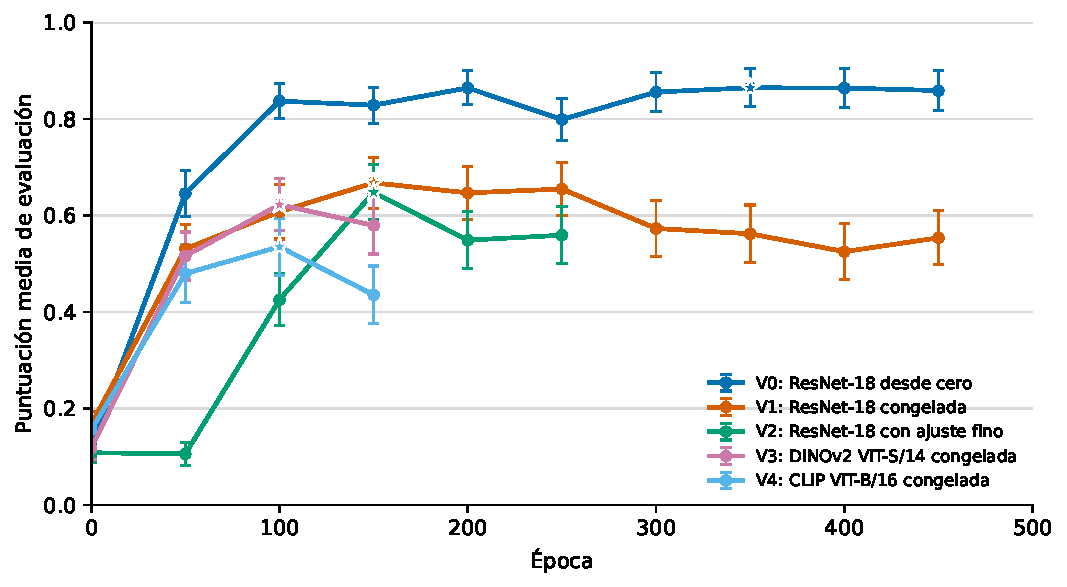
\includegraphics[width=0.74\linewidth]{evolucion_puntuacion_prueba.pdf}
  \src{Media sobre los \num{50} episodios reservados; barras de error estándar.
    Estrellas: punto de control seleccionado.}
\end{frame}

% ---------------------------------------------------------------- 9. tabla contrastes
\begin{frame}{Las cuatro diferencias frente a la línea base excluyen el cero}
  \begin{center}
  \begin{tabular}{l S[table-format=1.3] c l}
    \toprule
    & {Puntuación} & IC \SI{95}{\percent} de la diferencia & $p_{\mathrm{Holm}}$ \\
    \midrule
    \textbf{V0} desde cero & \bfseries 0.872 & {} & {} \\
    V1 ResNet congelada & 0.649 & [\num{0.170};\,\num{0.279}] & $<\num{1e-11}$ \\
    V2 ResNet ajustada  & 0.586 & [\num{0.228};\,\num{0.346}] & $<\num{1e-16}$ \\
    V3 DINOv2 congelada & 0.578 & [\num{0.234};\,\num{0.353}] & $<\num{1e-15}$ \\
    V4 CLIP congelada   & 0.490 & [\num{0.318};\,\num{0.444}] & $<\num{1e-19}$ \\
    \midrule
    V1 frente a V2  & \fade{0.063} & \fade{[\num{0.001};\,\num{0.124}]} &
      \fade{\num{0.09}--\num{0.13}} \\
    \bottomrule
  \end{tabular}
  \end{center}
  \src{Diferencias pareadas sobre las \num{200} condiciones del bloque disjunto, con el
    ruido de difusión sincronizado. Intervalos por \textit{bootstrap} BCa; los diez
    contrastes se corrigen por Holm.}
  \takeaway{Caídas de entre el \SI{26}{\percent} y el \SI{44}{\percent}. Entre congelar y
    ajustar, en cambio, no hay diferencia demostrable.}
\end{frame}

% ---------------------------------------------------------------- 10. perdidas
\begin{frame}{Las preentrenadas memorizan: la validación sube mientras el ajuste mejora}
  \centering
  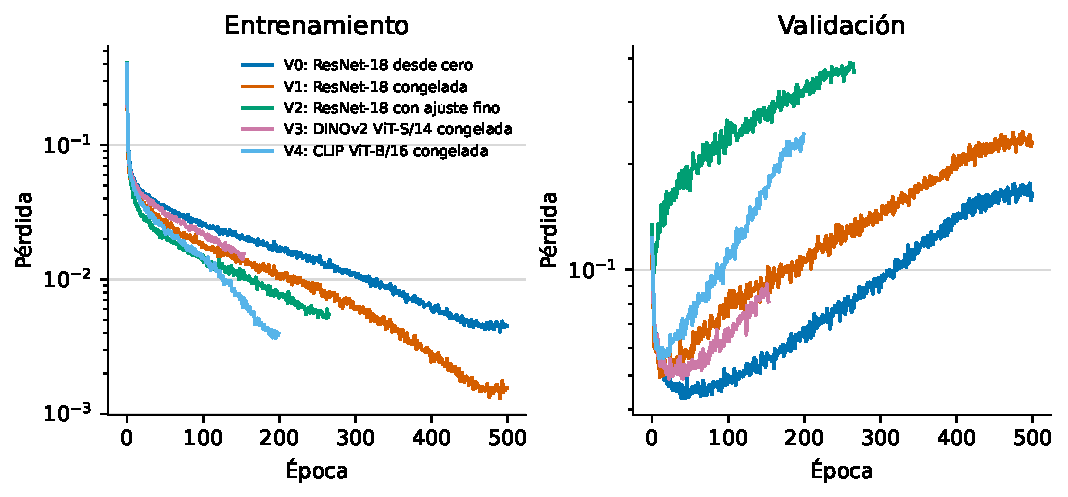
\includegraphics[width=0.78\linewidth]{evolucion_perdidas.pdf}
  \src{V1, entre las épocas \num{150} y \num{450}: entrenamiento
    \num{0.0145}$\rightarrow$\num{0.00166}, validación
    \num{0.0869}$\rightarrow$\num{0.2247}.}
\end{frame}

% ---------------------------------------------------------------- 11. coste
\begin{frame}{Congelar no abarata nada si obliga a subir la imagen a \num{224} píxeles}
  \begin{center}
  \begin{tabular}{l S[table-format=2.1] S[table-format=2.1] S[table-format=3.1]}
    \toprule
    & {Minutos por época} & {Factor} & {Horas totales} \\
    \midrule
    \textbf{V0} \fade{(\num{76} px)}  & \bfseries 1.6 & {--} & \bfseries 17.4 \\
    V1 \fade{(\num{224} px)}          & 5.3  & 3.3 & 96.5 \\
    V2 \fade{(\num{224} px)}          & 14.7 & 9.2 & 84.9 \\
    V3 \fade{(\num{224} px)}          & 2.3  & 1.4 & 10.9 \\
    V4 \fade{(\num{224} px)}          & 4.0  & 2.5 & 27.4 \\
    \bottomrule
  \end{tabular}
  \end{center}
  \src{Las horas totales no ordenan variantes: los presupuestos fueron distintos y V2 y V3
    se detuvieron antes. Total del experimento: \SI{237.1}{\hour} sobre una RTX 3070 Ti de
    \num{8} GB.}
  \takeaway{V1 entrena un \SI{4}{\percent} menos de parámetros y aun así cuesta tres veces
    más: manda la \hl{resolución de entrada}.}
\end{frame}

\section{Qué se puede afirmar}

% ---------------------------------------------------------------- 12. interpretacion
\begin{frame}{Por qué ImageNet no ayuda en un tablero sintético}
  \begin{itemize}
    \item Figuras geométricas sobre fondo uniforme: ni textura ni categorías.
    \item La tarea la decide la posición relativa de dos formas.
    \item V0 resuelve sobre \num{76} px reales; las preentrenadas interpolan la misma
          imagen hasta \num{224} px, sin añadir información.
  \end{itemize}
  \src{Coherente con R3M (Nair \emph{et al.}, 2022) y con DINOv3 (Egbe \emph{et al.}, 2025).
    Es una explicación plausible, no un mecanismo medido.}
\end{frame}

% ---------------------------------------------------------------- 13. limitaciones
\begin{frame}{Dónde falla este estudio}
  \begin{itemize}
    \item \hl{Una sola semilla de entrenamiento}: la unidad sobre la que se infiere es el
          artefacto, no la estrategia. Las \num{200} condiciones replican la evaluación,
          no el entrenamiento.
    \item Entre V0 y V1--V2 cambian \hl{varios factores a la vez}: pesos iniciales,
          resolución con recorte y normalización interna de la red.
    \item V1 y V2 ni siquiera parten del mismo archivo de pesos:
          \texttt{timm:resnet18.a1\_in1k} frente a \texttt{torchvision:IMAGENET1K\_V1}.
    \item Presupuestos desiguales y regla de parada adoptada \emph{después} de ver V0
          y V1.
  \end{itemize}
  \takeaway{Se comparan cinco artefactos concretos y su bloque visual completo, no
    estrategias de entrenamiento.}
\end{frame}

% ---------------------------------------------------------------- 14. cierre
\begin{frame}{Para llevarse a casa}
  \begin{enumerate}
    \item Con \num{90} demostraciones de Push-T, y sobre \num{200} condiciones nunca
          consultadas, la ResNet-18 desde cero ganó por entre \num{0.223} y \num{0.382}
          puntos, y además es la más barata por época.
    \item Ajustar los pesos preentrenados no aportó ventaja sobre congelarlos, y ese
          contraste no aísla la estrategia: los pesos de partida difieren.
    \item Siguiente paso, por orden: \hl{replicar con varias semillas de entrenamiento};
          después, entrenar desde cero a \num{224} px para separar los factores.
  \end{enumerate}
  \vfill
  {\color{tsMute}\small Bifurcación propia de \texttt{diffusion\_policy} ·
    \num{1621} épocas ejecutadas · \SI{237.1}{\hour} de GPU}
\end{frame}

% ================================================================== respaldo
\appendix

\begin{frame}[noframenumbering]{Respaldo}
  \centering{\color{tsMute}Material de apoyo para el turno de preguntas}
\end{frame}

\begin{frame}[noframenumbering]{Muestreo y horizonte deslizante}
  \[
    \Act{k-1} = \alpha\Big(\Act{k} - \gamma\,\rnet\big(\Obs,\Act{k},k\big) +
      \mathcal{N}(0,\sigma^2 I)\Big)
  \]
  \donde{$\alpha$, $\gamma$ y $\sigma$ los fija el planificador DDPM, con \num{100} pasos
    en entrenamiento e inferencia.}
  \begin{itemize}
    \item El ruido fresco de cada paso preserva los distintos modos de acción.
    \item Se predicen $T_p=\num{16}$ acciones y se ejecutan las $T_a=\num{8}$ primeras
          antes de replanificar.
  \end{itemize}
\end{frame}

\begin{frame}[noframenumbering]{Métrica de la tarea}
  \[
    s_j = \max_{1 \le t \le T} \min\!\left(\frac{c_{j,t}}{\tau},\, 1\right)
  \]
  \donde{$c_{j,t}$ es la fracción del área objetivo cubierta y $\tau=\num{0.95}$.}
  \begin{itemize}
    \item Se toma el máximo del episodio porque la pieza puede desplazarse después.
    \item Se reporta la media sobre \num{50} episodios, con su error estándar.
  \end{itemize}
\end{frame}

\begin{frame}[noframenumbering]{Media de las tres últimas evaluaciones}
  \centering
  \begin{tabular}{l S[table-format=1.3] S[table-format=1.3] S[table-format=3.2]}
    \toprule
    & {Mejor} & {Media últimas 3} & {ECM de la acción} \\
    \midrule
    V0 & 0.864 & 0.862 & 116.17 \\
    V1 & 0.668 & 0.547 & 147.31 \\
    V2 & 0.648 & 0.585 & 42.86 \\
    V3 & 0.622 & 0.572 & 314.78 \\
    V4 & 0.535 & 0.483 & 94.93 \\
    \bottomrule
  \end{tabular}
  \src{Cifras del \hl{conjunto de selección}, no de la prueba final: el máximo de una
    serie de evaluaciones es un estimador optimista. V2 logra el menor error sobre
    acciones del conjunto de datos y aun así no gana la tarea: precisión en cadena abierta
    y control en bucle cerrado no miden lo mismo.}
\end{frame}

\begin{frame}[noframenumbering]{Hiperparámetros comunes}
  \centering
  \begin{tabular}{ll}
    \toprule
    Parámetro & Valor \\
    \midrule
    Horizontes $T_p / T_o / T_a$ & \num{16} / \num{2} / \num{8} \\
    Pasos de difusión            & \num{100} (DDPM, varianza fija) \\
    Optimizador                  & AdamW, \num{1e-4}, decaimiento coseno \\
    Media móvil exponencial      & activada \\
    Tamaño de lote               & \num{64} (\num{32} en V4) \\
    Presupuesto                  & \num{500} épocas, parada anticipada \\
    Semilla                      & \num{42} \\
    \bottomrule
  \end{tabular}
  \src{Parada anticipada: sin superar el máximo en dos evaluaciones consecutivas y nunca
    antes de la época \num{200}. Solo llegó a aplicarse a V2.}
\end{frame}

\begin{frame}[noframenumbering]{Comprobación cualitativa, misma condición inicial}
  \begin{columns}[T,onlytextwidth]
    \begin{column}{0.49\textwidth}
      \centering V1 congelado, máximo \num{0.9544}\\[0.3em]
      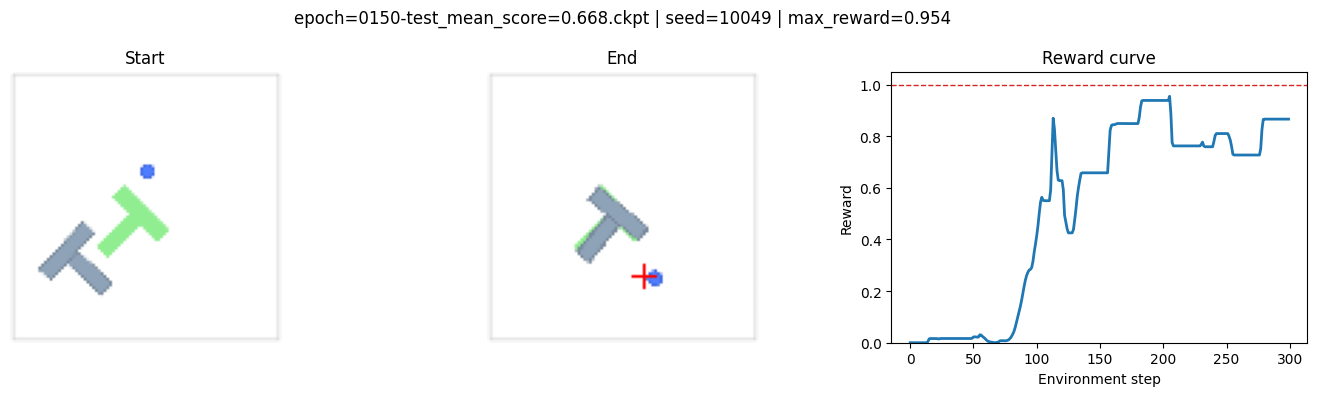
\includegraphics[width=\linewidth]{inferencia_v1.png}
    \end{column}
    \begin{column}{0.49\textwidth}
      \centering V2 ajuste fino, máximo \num{0.8818}\\[0.3em]
      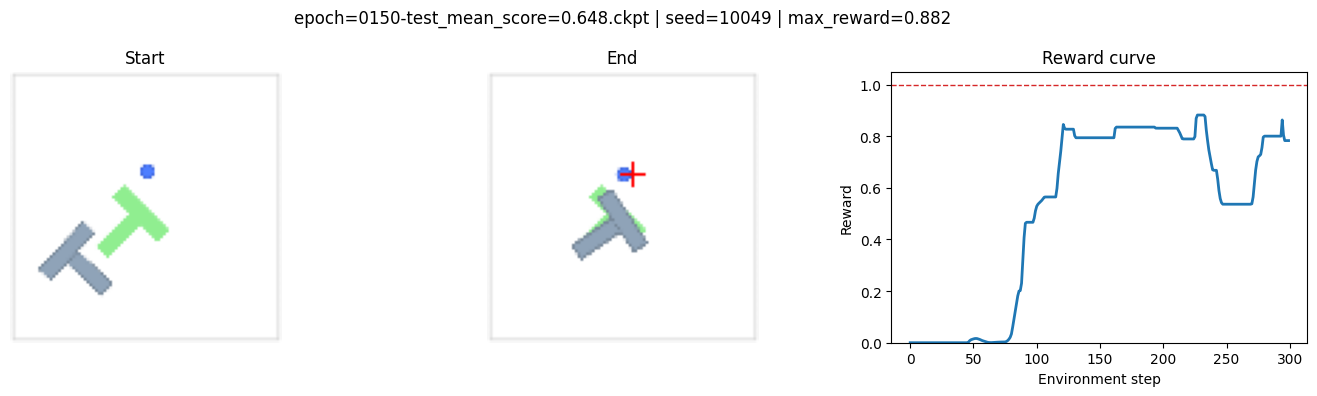
\includegraphics[width=\linewidth]{inferencia_v2.png}
    \end{column}
  \end{columns}
  \src{Semilla \num{10049}, fuera del intervalo oficial \num{100000}--\num{100049}. Un solo
    episodio: ilustra el comportamiento, no estima el rendimiento medio.}
\end{frame}

\begin{frame}[noframenumbering]{Trabajo futuro, con su coste}
  \begin{itemize}
    \item Completar V3 y V4: ¿el problema es ImageNet o todo preentrenamiento ajeno a
          la robótica?
    \item Desde cero a \num{224} px sin recorte, unas \SI{85}{\hour}; a \num{96} px sin
          recorte, unas \SI{17}{\hour}.
    \item Semillas \num{43} y \num{44} sobre las variantes seleccionadas.
    \item Evaluar sobre semillas disjuntas de las de selección.
  \end{itemize}
\end{frame}

\end{document}
